Como apresentado por \citeonline{jesus2023inteligencia}, 
redes neurais são estruturas baseadas em grafos, representadas em camadas; 
cada camada é composta por nós, denominados neurônios, e arestas, 
denominadas sinapses. A estrutura básica de uma rede neural possui três camadas: 
entrada, camada intermediária e saída, que são, respectivamente, responsáveis 
por executar as funções de receber os dados externos, 
processar os dados e entregar o resultado.

A técnica de redes neurais apresenta derivações amplamente utilizadas como alicerce 
no desenvolvimento de sistemas baseados em Deep Learning.

\begin{figure}[H]
    \centering
    \caption{Representação Visual em Grafo da estrutura básica de uma Rede Neural}
    \label{fig:est_bas_nn}
    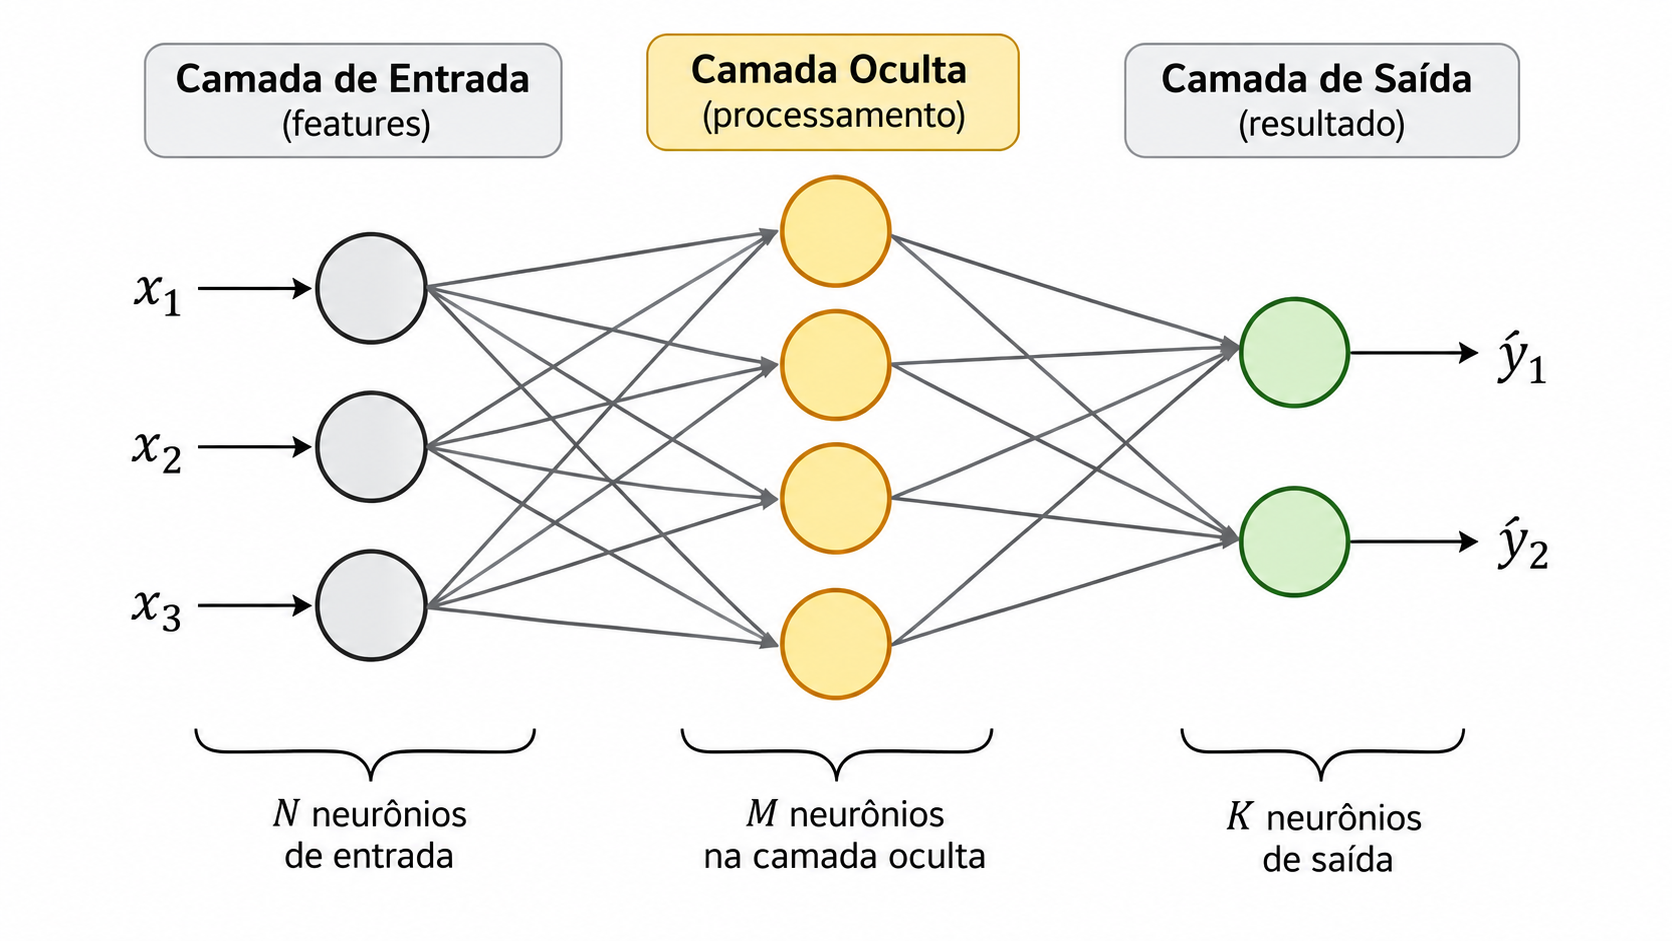
\includegraphics[width=0.85\textwidth]{sections/imagens/Grafo_Redes_Neurais.png}
    \small
    % Imagem com origem no Gemini
\end{figure}


\subsubsubsection{Redes Neurais Convolucionais}

Atualmente, as redes neurais convolucionais são amplamente aplicadas em processamento de dados não estruturados, 
como imagens, vídeos e áudios. Tal técnica tem como característica o 
processamento de pequenos trechos de dados por vez, ao contrário 
de outras técnicas que tentam realizar o processamento de forma atômica 
\cite{jesus2023inteligencia}.

Como apresentado por \citeonline{Atika2022ImageSegmentation}, 
o desenvolvimento de uma \gls{cnn} inicia-se pela definição da arquitetura em implementação. 
Tal técnica abrange uma vasta quantidade de arquiteturas que foram 
desenvolvidas para auxiliar e alcançar melhores resultados para 
determinados requisitos do software.

\subsubsubsection{Camadas que Constituem uma CNN} 
Uma \gls{cnn} é constituída por três principais camadas: camada de entrada de dados, 
camada de saída, também denominada camada densa, 
na qual cada um de seus neurônios está conectado à camada anterior, e diversas outras 
camadas intermediárias, 
denominadas por alguns autores camadas ocultas \cite{ayeni2022convolutional}. 

As camadas intermediárias de uma CNN 
apresentam comportamento de aprofundamento em reconhecimento de abstrações a cada camada sobreposta, 
de tal forma que as camadas iniciais são responsáveis por identificar traços, 
contornos, linhas etc., 
enquanto as camadas finais possuem a responsabilidade de identificar objetos, 
rostos e valores, por exemplo. 
Tais camadas são desenvolvidas com a intercalação de camadas de convolução e pooling (agrupamento), 
de forma que cada entrada de uma camada é a saída da camada anterior.

\paragraph{Camada Convolucional}
Como \citeonline{ayeni2022convolutional} explica, 
a camada convolucional é a camada responsável por processar imagens de forma 
a encontrar padrões ao aplicar um filtro (kernel/neurônio) a cada trecho 
da imagem de entrada, denominado campo receptivo. 
O neurônio é responsável por aplicar operações de multiplicação sobre o campo receptivo, 
gerando um único valor para cada trecho de imagem processado, 
e, posteriormente, os valores calculados pelos neurônios são 
armazenados em uma estrutura de três dimensões \cite{ayeni2022convolutional}.

A conversão da imagem para escala de cinza antes 
do processamento por uma \gls{cnn} é justificada 
por reduzir a complexidade cromática do padrão 
\gls{rgb} (três canais) para um canal único, 
o que impacta diretamente a profundidade dos kernels e o volume 
de parâmetros da primeira camada da rede 
\cite{ayeni2022convolutional}.

\paragraph{Camada de Pooling}
Segundo \citeonline{ayeni2022convolutional}, 
a camada de pooling possui a responsabilidade de filtrar características predominantes 
encontradas na camada de convolução. 
Tal camada possui a importantíssima função de otimizar processamento, 
descartando dados menos significativos 
e mitigando o fenômeno de overfitting.
As camadas de pooling possuem diversas derivações, que são 
escolhidas e implementadas a fim de otimizar resultados alcançados pelo modelo, 
mas a derivação mais aplicada sobre CNNs é a Max Pooling.

A operação de pooling reduz a resolução 
espacial dos mapas de características 
gerados pela camada convolucional, 
utilizando tipicamente uma janela de 
varredura (filtro) de $2 \times 2$.

\paragraph{Camada Totalmente Conectada}
Como \citeonline{ayeni2022convolutional} explica, 
a camada denominada Fully-Connected (Totalmente Conectada) possui a função de interpretar 
abstrações mais complexas da imagem e classificá-las. 
Essa camada possui todos os seus parâmetros conectados 
com os parâmetros da camada anterior, 
corriqueiramente resultando em um número de nós de saída 
igual à quantidade de classes de classificação.
